


\documentclass[aspectratio=169,xcolor=dvipsnames]{beamer}
%\usetheme{SimplePlus}

\usepackage{hyperref}
\usepackage{graphicx} % Allows including images
\usepackage{booktabs} % Allows the use of \toprule, \midrule and \bottomrule in tables

%----------------------------------------------------------------------------------------
%	TITLE PAGE
%----------------------------------------------------------------------------------------
\title[Flowmåling] {Strømningsmåling}

%\subtitle{Subtitle}

\author[Fred-Olav] {Fred-Olav Mosdal}

\institute[Gand VGS] % Your institution as it will appear on the bottom of every slide, may be shorthand to save space
{
    Gand VGS \\
    VG3 Automasjon
}
\date{\today} % Date, can be changed to a custom date
\begin{document}
\maketitle

\begin{frame}
	\frametitle{Strømningsvakter}
\end{frame}

\begin{frame}
	\frametitle{Bruk av strømningsvakter}

	\begin{columns}
		\begin{column}{0.5\textwidth}
			\begin{itemize}
				\item Tørrkjøring
				\item manglende kjøling
				\item manglende smøring
			\end{itemize}

			
		\end{column}

		\begin{column}{0.5\textwidth}
			$$\includegraphics[width=1\textwidth]{../output/noGPLimages/strømningsvakt.png}$$
			\end{column}
		\end{columns}
\end{frame}
\begin{frame}
	\frametitle{Kalorimetrisk prinsipp}

	\begin{columns}
		\begin{column}{0.5\textwidth}
					Måler hvor mye energi som går med på å holde teperaturen i et varmeelement.

			
		\end{column}

		\begin{column}{0.5\textwidth}
			$$\includegraphics[width=1\textwidth]{../output/noGPLimages/strømning01.png}$$
			\end{column}
		\end{columns}
\end{frame}


\begin{frame}
	\frametitle{Mekanisk strømningsvakt}

			$$\includegraphics[width=1\textwidth]{../output/noGPLimages/strømning02.png}$$
\end{frame}
\begin{frame}
	\frametitle{Strømningsvakt basert på trykkfall}

			$$\includegraphics[height=0.8\textheight]{../output/noGPLimages/strømning03.png}$$
\end{frame}
\begin{frame}
	\frametitle{Strømningsvakt basert på endring av frekvens}

			$$\includegraphics[height=0.8\textheight]{../output/noGPLimages/strømning04.png}$$
\end{frame}
\begin{frame}
	\frametitle{Massestrøm med veieteknikk}

$$A_1 \overline{v_1} = A_2 \overline{v_2}$$
\end{frame}
\begin{frame}
	\frametitle{Doserbåndvekt}

$$\includegraphics{flow66.eps}$$

\end{frame}
\begin{frame}
	\frametitle{Doserbåndvekt}

$\includegraphics[width=4in]{flow81.eps}$
\end{frame}
\begin{frame}
	\frametitle{Doserbåndvekt}

			$$\includegraphics[height=0.8\textheight]{../output/noGPLimages/strømning05.png}$$
\end{frame}
\begin{frame}
	\frametitle{Beholdervekt}

			$$\includegraphics[height=0.8\textheight]{../output/noGPLimages/strømning06.png}$$
\end{frame}

\end{document}
